\documentclass[conference, onecolumn]{IEEEtran}
\IEEEoverridecommandlockouts
\usepackage{cite}
\usepackage{amsmath,amssymb,amsfonts}
\usepackage{algorithmic}
\usepackage{graphicx}
\usepackage{textcomp}
\usepackage{xcolor}
\usepackage{flushend}
\def\BibTeX{{\rm B\kern-.05em{\sc i\kern-.025em b}\kern-.08em
    T\kern-.1667em\lower.7ex\hbox{E}\kern-.125emX}}
\begin{document}

\title{IOT102 IoT based Smart Waste Management System\\
}

\author{
1\textsuperscript{st} Lam Quoc Phong, 2\textsuperscript{nd} Le Tran Minh Dat, 3\textsuperscript{rd} Lam Tien Hung, 4\textsuperscript{th} Phan Nhat Minh and Duc Ngoc Minh Dang\\
FPT University, Ho Chi Minh Campus, Vietnam\\
\{phonglqse183161, datltmse170095, minhpnse172531, hungltse170216\}@fpt.edu.vn, and ducdnm2@fe.edu.vn}
\maketitle

\section{Abstract}
This report investigates the plan and execution of a brilliant dustbin framework utilizing Blynk 2.0 and NodeMCU ESP8266 microcontrollers. The framework use ultrasonic sensors to quantify squander levels and naturally controls the cover opening in view of pre-characterized limits. Blynk gives an easy to understand connection point to observing burn through levels progressively, getting warnings when the container is full, and somewhat controlling the top. This report subtleties the equipment parts, programming advancement, and functionalities of the savvy dustbin, featuring its expected advantages for further developed squander the board effectiveness and diminished natural effect.


\section{Introduction}
The management of waste is an important problem that affects cities all over the world. Customary waste assortment techniques are many times wasteful and impractical, prompting ecological contamination and general wellbeing gambles. To address these difficulties, imaginative arrangements like savvy dustbins are arising, utilizing the force of the Web of Things (IoT) to upgrade squander assortment and further develop generally squander the executives methodologies.

This report dives into the improvement of a shrewd dustbin utilizing Blynk 2.0 and NodeMCU ESP8266. We investigate the coordination of equipment parts like ultrasonic sensors and servo engines with the Blynk IoT stage to accomplish constant checking and control of waste levels. The smart dustbin's design process, hardware setup, software development, and functionality will all be discussed in detail in this report, highlighting its potential advantages for better waste management in urban environments.

\begin{figure}[htbp]
\centerline{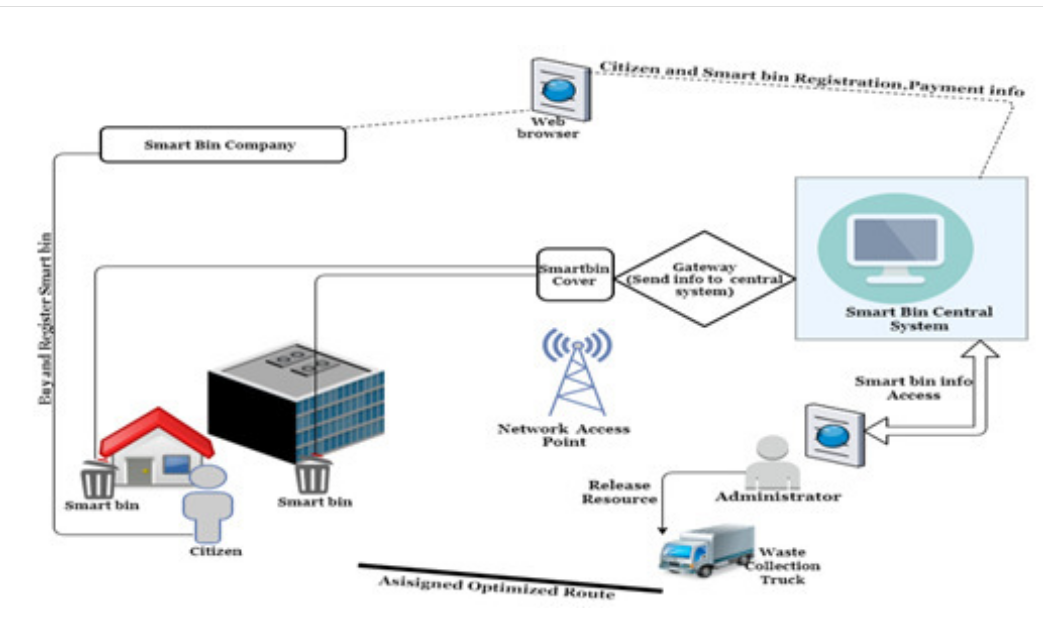
\includegraphics[width=3.8 in]{figure.png}}
\caption{This is an example of a figure.}
\label{fig}
\end{figure}

\section{Main proposal}
The research topic "Smart Dustbin with IoT using Blynk 2.0 and ESP32/NodeMCU ESP8266" has a lot of practical, current, and scientific importance. It tends to the squeezing difficulties of waste administration, lines up with the worldwide pattern towards savvy urban communities, and adds to the progression of IoT innovation in the field. The study has the potential to change the way waste management is done, increase productivity, and encourage environmental sustainability.\\

\subsection{System models and block diagram}

The smart dustbin system comprises the following hardware components:

NodeMCU ESP8266 microcontroller: Processes data from sensors and controls the system.

Ultrasonic sensor: Measures the distance to the top of the waste pile, determining the waste level.

Servo motor: Automatically opens and closes the lid based on pre-defined thresholds.

Breadboard and jumper wires: Connect the various components.

Power supply: Provides the necessary voltage to operate the system.\\

\begin{center}
\centerline{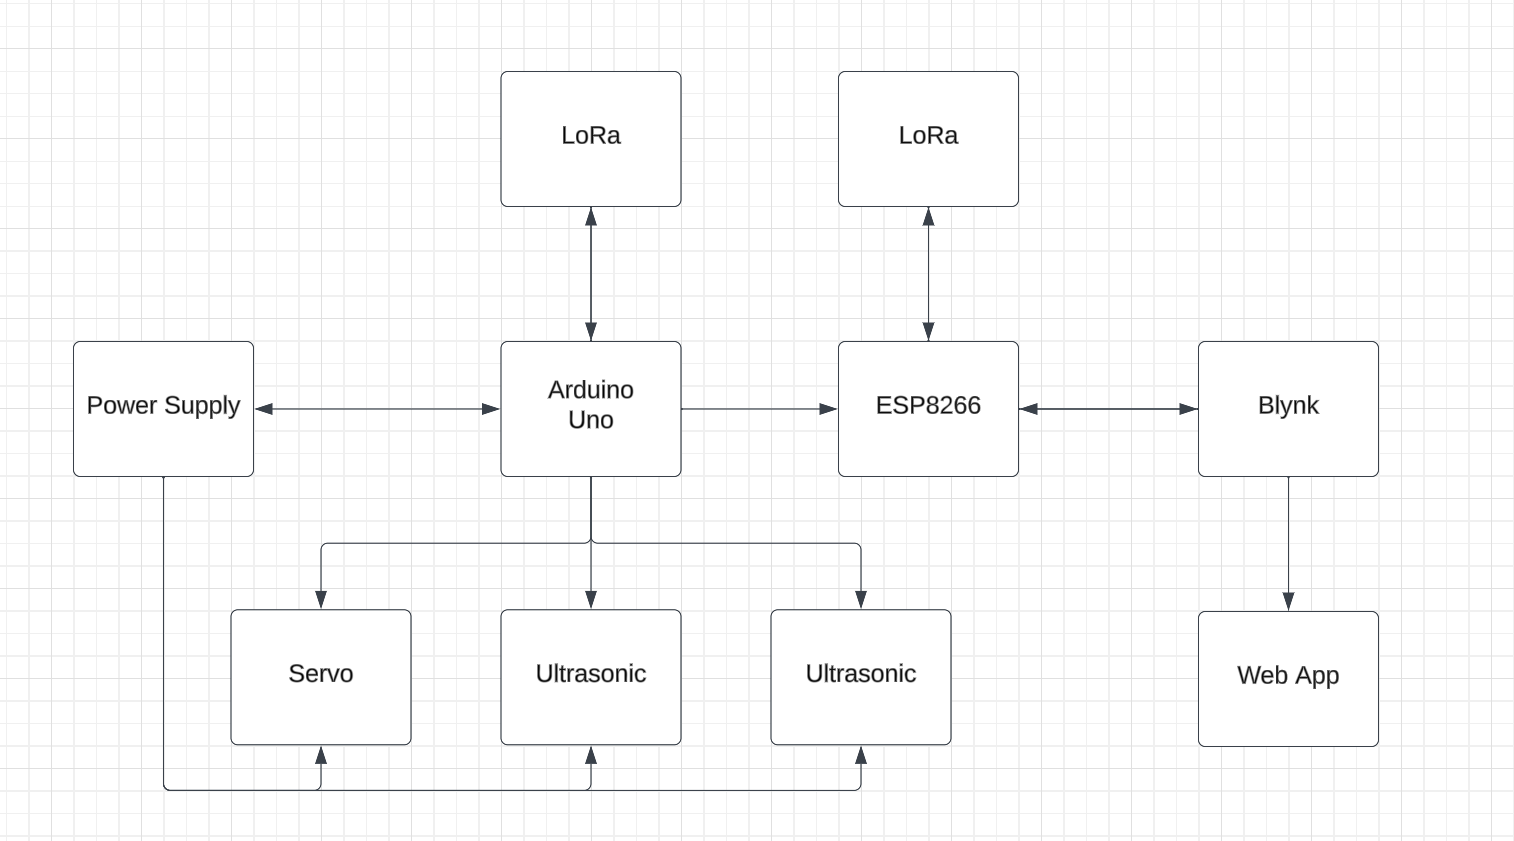
\includegraphics[width=3.8 in]{Block_diagram.png}}
A.1 The Block Diagram of the System
\end{center}



\subsection{Components and peripheral devices}

B.1 ESP8266:\\
The ESP8266 is a low-cost WiFi microchip with built-in networking capabilities, popular for IoT projects. It's easy to use, versatile, and supported by a large community. Explore its potential for home automation, wearables, robotics, and more!\\
\centerline{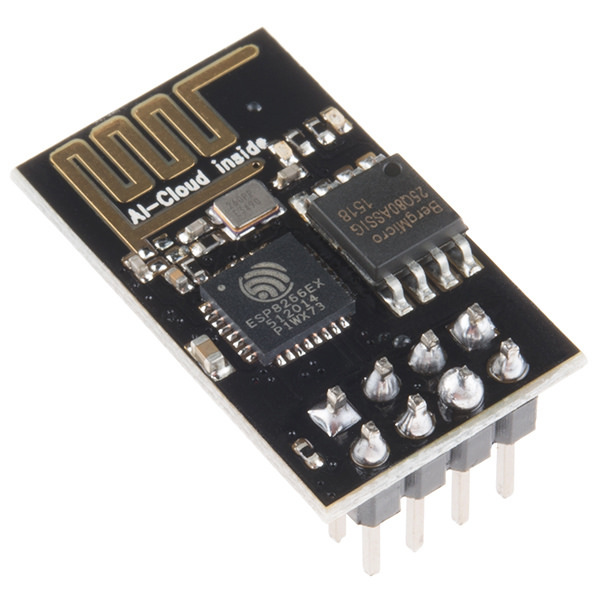
\includegraphics[width=3.8 in]{esp8266}}\\



B.2 Breadboard:\\
The BreadBoard, also known as a solderless breadboard or protoboard, is a temporary workspace for building electronic circuits. It allows you to easily connect components without soldering, making it perfect for prototyping and experimenting. Its rows and columns of holes are interconnected internally, enabling quick and flexible circuit creation. It's a crucial tool for beginners and experienced makers alike.\\
\centerline{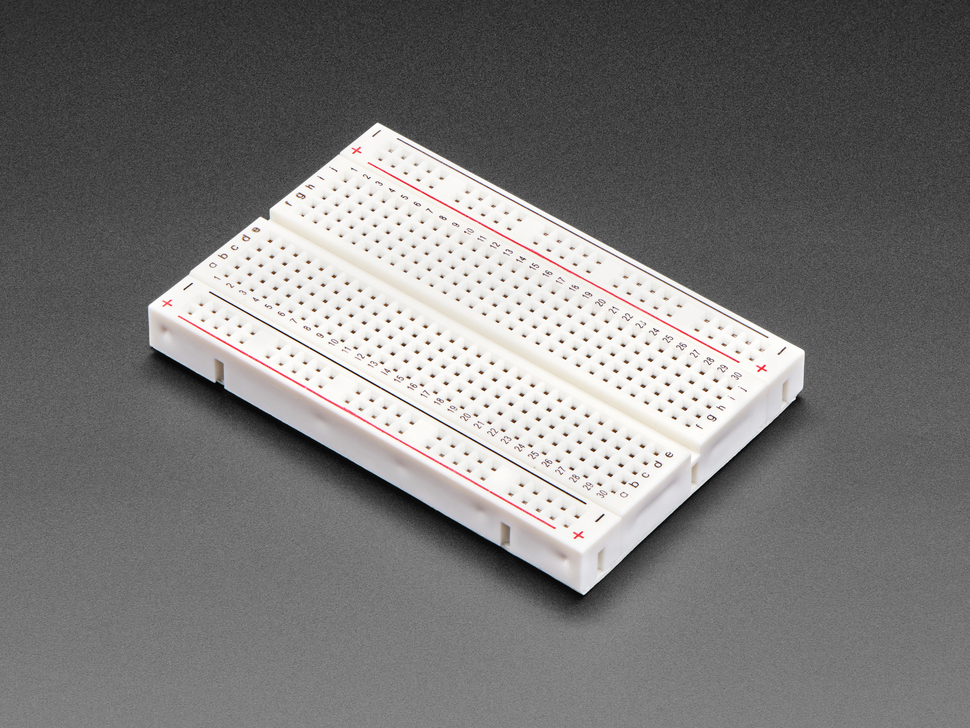
\includegraphics[width=3.8 in]{breadboard.png}}\\



B.3 Micro Controller Arduino:\\
Arduino is an open-source platform for creating electronics projects. It combines easy-to-use hardware boards and software that allows you to program micro controllers to read sensors, control lights, motors, and other devices. It's popular for beginners and experts alike for its affordability, versatility, and large community.\\
\centerline{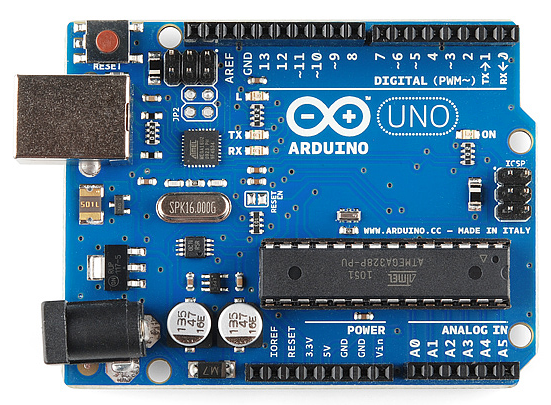
\includegraphics[width=3.8 in]{arduino}}\\



B.4 LoRa:\\
A LoRa module is a compact hardware component containing all the electronics needed to utilize LoRa technology. It integrates a LoRa transceiver chip, antennas, and supporting circuitry onto a single board, making it easy to add long-range wireless communication capabilities to your projects.\\
\centerline{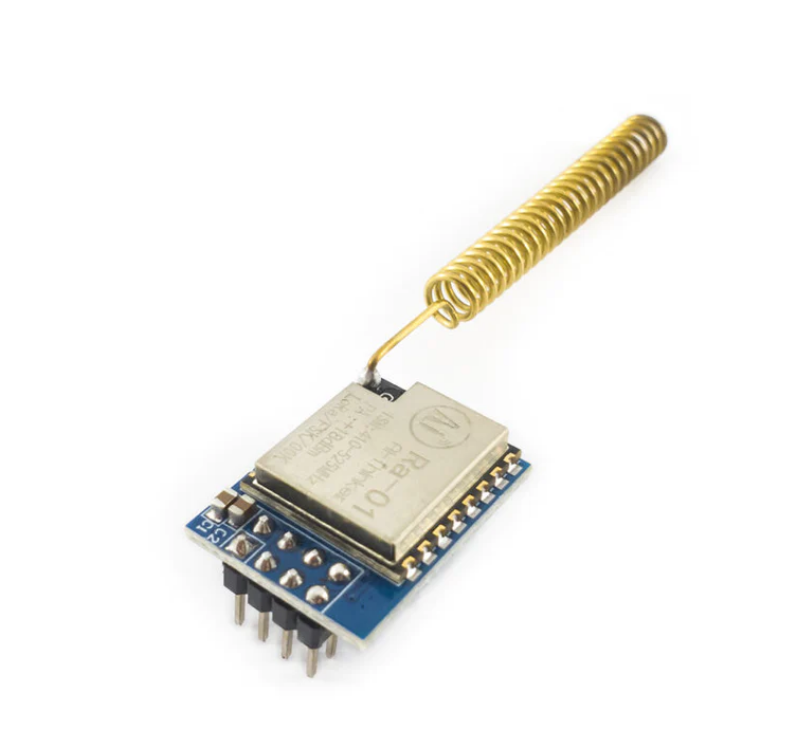
\includegraphics[width=3.8 in]{lora}}\\



B.5 Servo Motor:\\
Servo engines assume an essential part in the realm of IoT, empowering exact and controlled development in different applications. Not at all like customary DC engines that pivot ceaselessly, servos can be situated at explicit points and stand firm on their foothold with surprising precision. In this connected world, they are ideal for developing dynamic and interactive devices.\\
\centerline{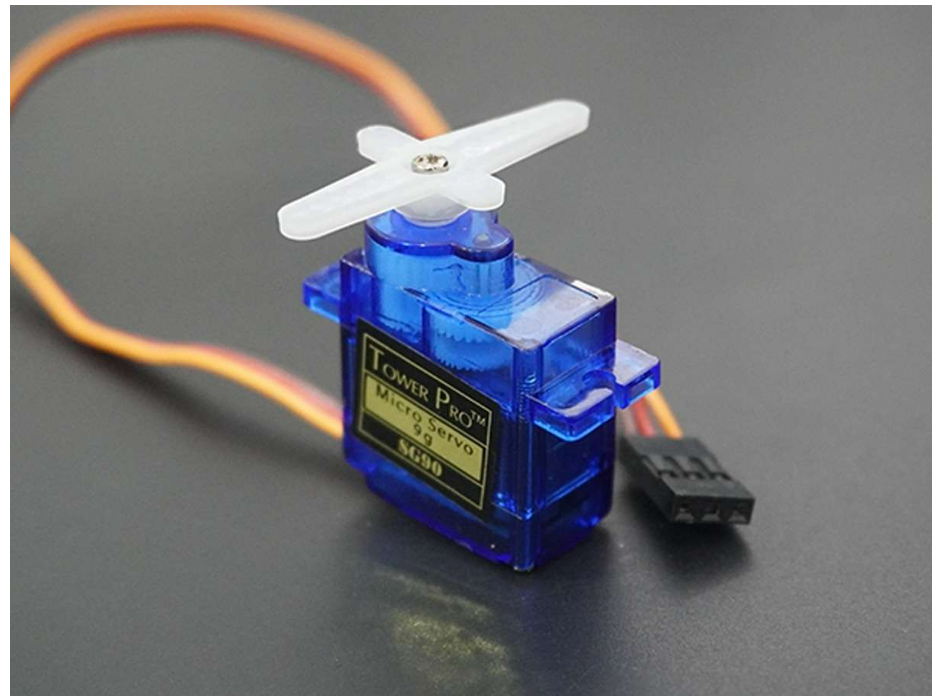
\includegraphics[width=3.8 in]{servo}}\\



B.6 Jump Wires: \\
Jump wires, also known as jumper wires or Dupont wires, are a vital component in the world of IoT (Internet of Things). These simple yet versatile wires play a crucial role in connecting various components, facilitating communication and data transfer between them. In the ever-evolving landscape of IoT, where miniaturization and flexibility are key, jump wires offer an effective and accessible solution for prototyping and building diverse IoT applications.\\
\centerline{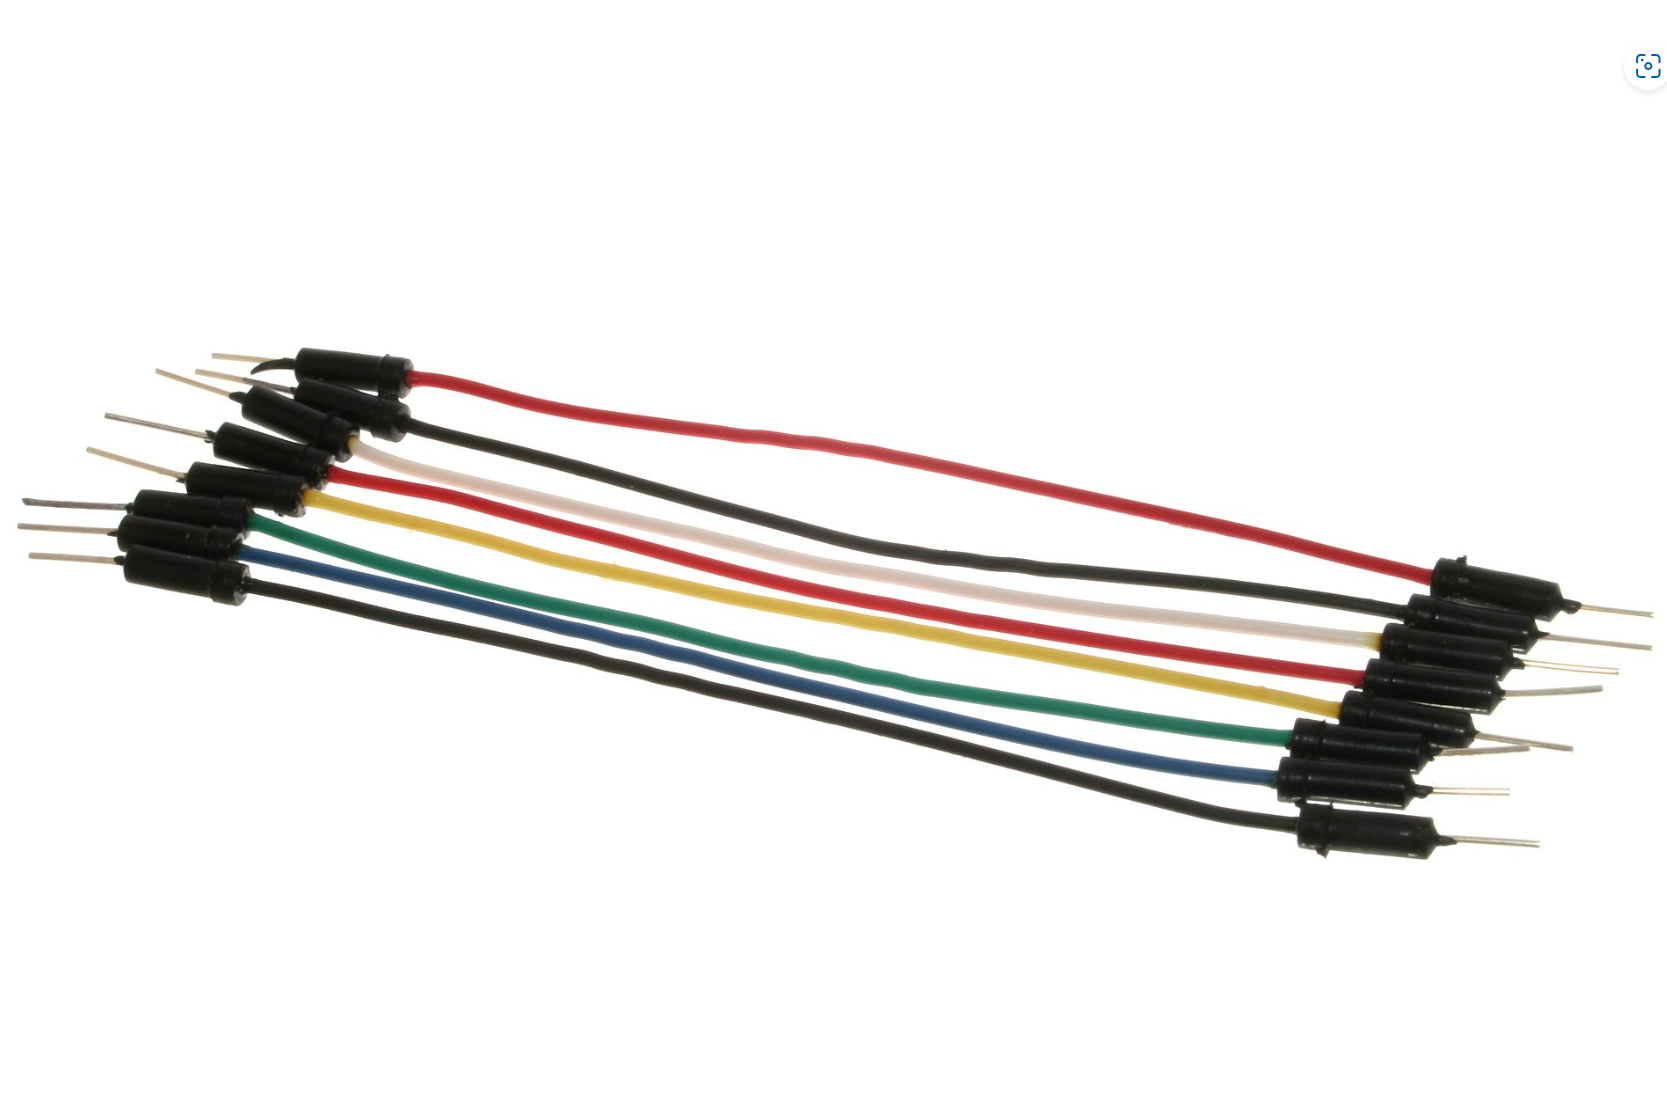
\includegraphics[width=3.8 in]{jump}}\\

B.7 Ultra Sensor Range Finder:\\
Ultrasonic reach locater sensors are a sort of sensor that utilization sound waves to quantify the distance to an item. They are generally utilized in different applications, including advanced mechanics, hindrance aversion, stopping help, and modern robotization.\\
\centerline{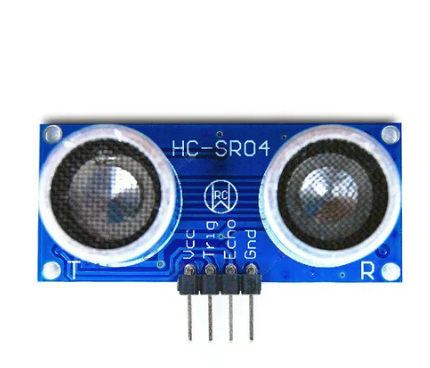
\includegraphics[width=3.8 in]{sensor}}\\


\subsection{Software programming}


Arduino IDE: Provide an overview of the Arduino Integrated Development Environment (IDE) and its role in programming the microcontroller. Explain how to install the IDE and set up the necessary board configuration for ESP32 or NodeMCU ESP8266.

Blynk 2.0 platform: Describe the Blynk 2.0 platform and its features for creating IoT applications. Discuss the advantages of using Blynk for rapid prototyping and its user-friendly interface for designing the user interface and configuring data communication.

Blynk library for NodeMCU ESP8266: Explain how to install the Blynk library in the Arduino IDE and how to use it for establishing communication between the microcontroller and the Blynk platform.

Libraries for interfacing with the ultrasonic sensor: Identify the specific libraries required to interface with the ultrasonic sensor. Provide instructions on how to install and use these libraries in the Arduino IDE.\\


C.1 Source Code:\\
define BLYNK_PRINT Serial \\
define BLYNK_TEMPLATE_ID "TMPL6bP4FNpNI"\\
define BLYNK_TEMPLATE_NAME "PROJECT"\\
define BLYNK_AUTH_TOKEN "BvH3H3framvDOR6LVOmWDs9oAELIIZ9D"\\
include <LoRa.h>\\
include <ESP8266WiFi.h>\\
include <BlynkSimpleEsp8266.h>\\
include <NewPing.h>\\
include <NTPClient.h>\\             
include <TimeLib.h>\\  

define LORA_SS_PIN D8\\
define LORA_RST_PIN D4\\
define LORA_DI0_PIN D1\\
define CLOSE_DISTANCE 10\\

char auth[] = BLYNK_AUTH_TOKEN;\\
char ssid[] = "Garage Coffee"; // your wifi name\\
char pass[] = "garageopen24h"; // passwifi\\
int v0 = 0; // Status garbage\\
//OFF\\
int v1 = 0; // LOCK\\

//Lock\\
BLYNK_WRITE(V0) {\\
  v0 = param.asInt();\\
}\\

BLYNK_WRITE(V1) {\\
  v1 = param.asInt();\\
}\\

//Trans\\
void commonSetup() {\\
  Serial.begin(115200);\\
  Blynk.begin(auth, ssid, pass);\\
  while (!Serial);\\
 
  LoRa.setPins(LORA_SS_PIN, LORA_RST_PIN, LORA_DI0_PIN);\\
  if (!LoRa.begin(433E6)) {\\
    Serial.println("LoRa init failed. Check your connections!");\\
    while (1);\\
  } else {\\
    Serial.println("LoRa init successful.");\\
    LoRa.setTxPower(22);\\
  }\\\\
}\\

void sendToBlynk(int value1, int value2) {\\
  Blynk.virtualWrite(V2, value1);\\
  Blynk.virtualWrite(V3, value2);\\
//  Blynk.virtualWrite(V4, value3);\\
  
}\\

void setup() {\\
  //Mode transmitter\\
  if (v0 == 0) {\\
    commonSetup();\\
  }\\
  //Mode receiver\\
  else {\\
    Serial.println("\n>>Receiver");\\
    Serial.begin(115200);\\
    Blynk.begin(auth, ssid, pass);\\
    while (!Serial);\\

    LoRa.setPins(LORA_SS_PIN, LORA_RST_PIN, LORA_DI0_PIN);\\
    if (!LoRa.begin(433E6)) {\\
      Serial.println("LoRa init failed. Check your connections!");\\
      while (1);\\
    } else {\\
      Serial.println("LoRa init successful.");\\
      LoRa.setTxPower(20);\\
      LoRa.receive();\\
    }\\
  }\\
}\\

void loop() {\\
  Blynk.run();\\
  if (v0 == 0 && LoRa.beginPacket()) {\\
    String dataToSend = String(v0) + ", " + String(v1);\\
    LoRa.println(dataToSend);\\
    LoRa.endPacket();\\
    Serial.println("Data sent from ESP8266: " + dataToSend);\\
    delay(1000);\\
  }\\
  // Receive data from LoRa module\\
  else if (v0 != 0 && LoRa.parsePacket()) {\\
    String receivedData = "";\\
    while (LoRa.available()) {\\
      receivedData += (char)LoRa.read();\\
    }\\
    char delimiter[] = ", ";\\
    char* token = strtok((char*)receivedData.c_str(), delimiter);\\

    String data1 = token; // Percentage_Garbage_FULL\\
    token = strtok(NULL, delimiter);\\
    String data2 = token; // IS_OPEN OR NOT\\
    token = strtok(NULL, delimiter);\\
    String data3 = token;\\
    int value1 = data1.toInt();\\
    int value2 = data2.toInt();\\
//    int value3 = data3.toInt();\\
    Serial.println("Data receive >> ");\\
    if (value2 == 1) {\\
      Serial.println("Percentage: " + data1 + ", Garbage OPEN");\\
    } else {\\
      Serial.println("Percentage: " + data1 + ", Garbage NOT_OPEN");\\
    }\\

    sendToBlynk(value1, value2);\\
  }\\
  delay(1);\\
}\\


C.2 Source Code Transmitter:\\
include <SPI.h>\\
include <LoRa.h>\\
include <Servo.h>\\
include <NewPing.h>\\

define TRIGGER_PIN_1 7\\
define ECHO_PIN_1 6\\
define TRIGGER_PIN_2 5\\
define ECHO_PIN_2 4\\
define SERVO_PIN 3\\
define LORA_SS_PIN 10\\
define LORA_RST_PIN 9\\
define LORA_DI0_PIN 2\\
define CLOSE_DISTANCE 10\\

NewPing sonar1(TRIGGER_PIN_1, ECHO_PIN_1);\\
NewPing sonar2(TRIGGER_PIN_2, ECHO_PIN_2);\\
Servo myServo;\\

int binFullCount = 0;\\

void setup() {\\
  Serial.begin(115200);\\

  LoRa.setPins(LORA_SS_PIN, LORA_RST_PIN, LORA_DI0_PIN);\\
  myServo.attach(SERVO_PIN);\\
  if (!LoRa.begin(433E6)) {\\
    Serial.println("LoRa init failed. Check your connections!");\\
    while (1);\\
  }\\
  Serial.println("LoRa init successful.");\\
}

void loop() {\\
  int distance1 = sonar1.ping_cm();\\
  int distance2 = sonar2.ping_cm();\\

  bool isHumanNearby = false;\\
  if (distance1 <= CLOSE_DISTANCE) {\\
    isHumanNearby = true;\\
    myServo.write(90);\\
  } else {\\
    isHumanNearby = false;\\
    myServo.write(0);\\
  }\\

  float emptyDistance = 30.0;\\
  float fullDistance = 5.0;\\
  float currentDistance = distance2;\\
  float percentage = 100.0 - ((currentDistance - fullDistance) / (emptyDistance - fullDistance)) * 100.0;\\
  percentage = constrain(percentage, 0, 100);\\

  // Construct the data to send via LoRa\\
  String dataToSend = String(percentage) + ", " + String(isHumanNearby);\\
  
  // Send the data via LoRa\\
  LoRa.beginPacket();\\
  LoRa.print(dataToSend);\\
  LoRa.endPacket();\\
  
  // Print the sent data to the Serial Monitor\\
  Serial.println("Sent 1 & 2: " + dataToSend);\\
  
  delay(1000);\\
}\\




\subsection{Programming Flowchart}
The ultrasonic sensors mounted to the top of the dustbin continuously measure the distance to the top of the trash pile. They send these readings over the LoRa link to the main Arduino.

The Arduino monitors the distances received from the two ultrasonic sensors. Based on predefined thresholds, it determines if the trash level is low, medium, high or full.

The Arduino reports the trash level status to Blynk cloud service using the WiFi/GPRS connection.

The Blynk app displays the status of each dustbin to the operator, allowing monitoring from anywhere. Notifications can also be setup for each dust bin status.

When the status shows full for a dustbin, the operator can use the Blynk app to remotely trigger that dustbin to open its servo-operated lid.
Once the trash is emptied by the sanitary staff, the lid can be remotely closed as well from the Blynk app.

The updated status then reflects the new trash level for that dustbin based on continuous measurement by the ultrasonic sensors.\\

\begin{center}
\centerline{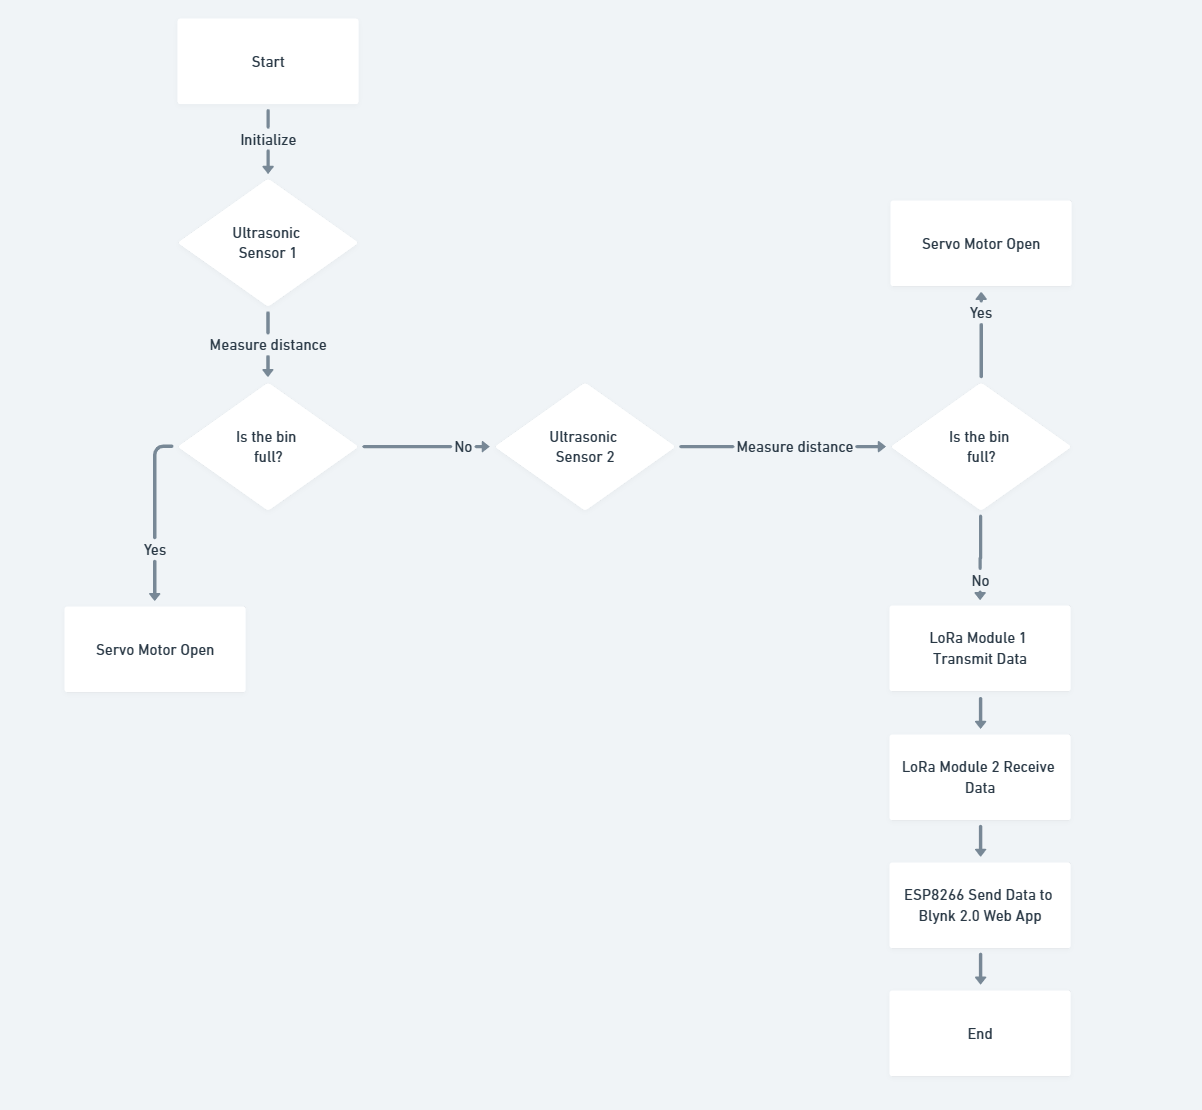
\includegraphics[width=3.8 in]{flowchart.png}}
D.1 Algorithm Flowchart of The System
\end{center}

\section{Results and discussion}
The exploration strategies for the report on the brilliant dustbin framework included writing survey, framework plan, model turn of events, Blynk 2.0 mix, assessment and testing, information examination, and documentation. These strategies were utilized to guarantee an orderly and thorough way to deal with the examination, bringing about a factual report on the execution and assessment of the savvy dustbin framework.\\

\subsection{Prototype Implementation}
The model execution effectively showed the practicality of a savvy dustbin framework using Blynk 2.0 and NodeMCU ESP8266. The framework gives constant waste level checking, programmed cover control, remote access, and easy to understand interface, displaying its true capacity for further developing waste administration effectiveness and adding to a cleaner climate.\\

\subsection{Experimental Results}
\begin{center}
\centerline{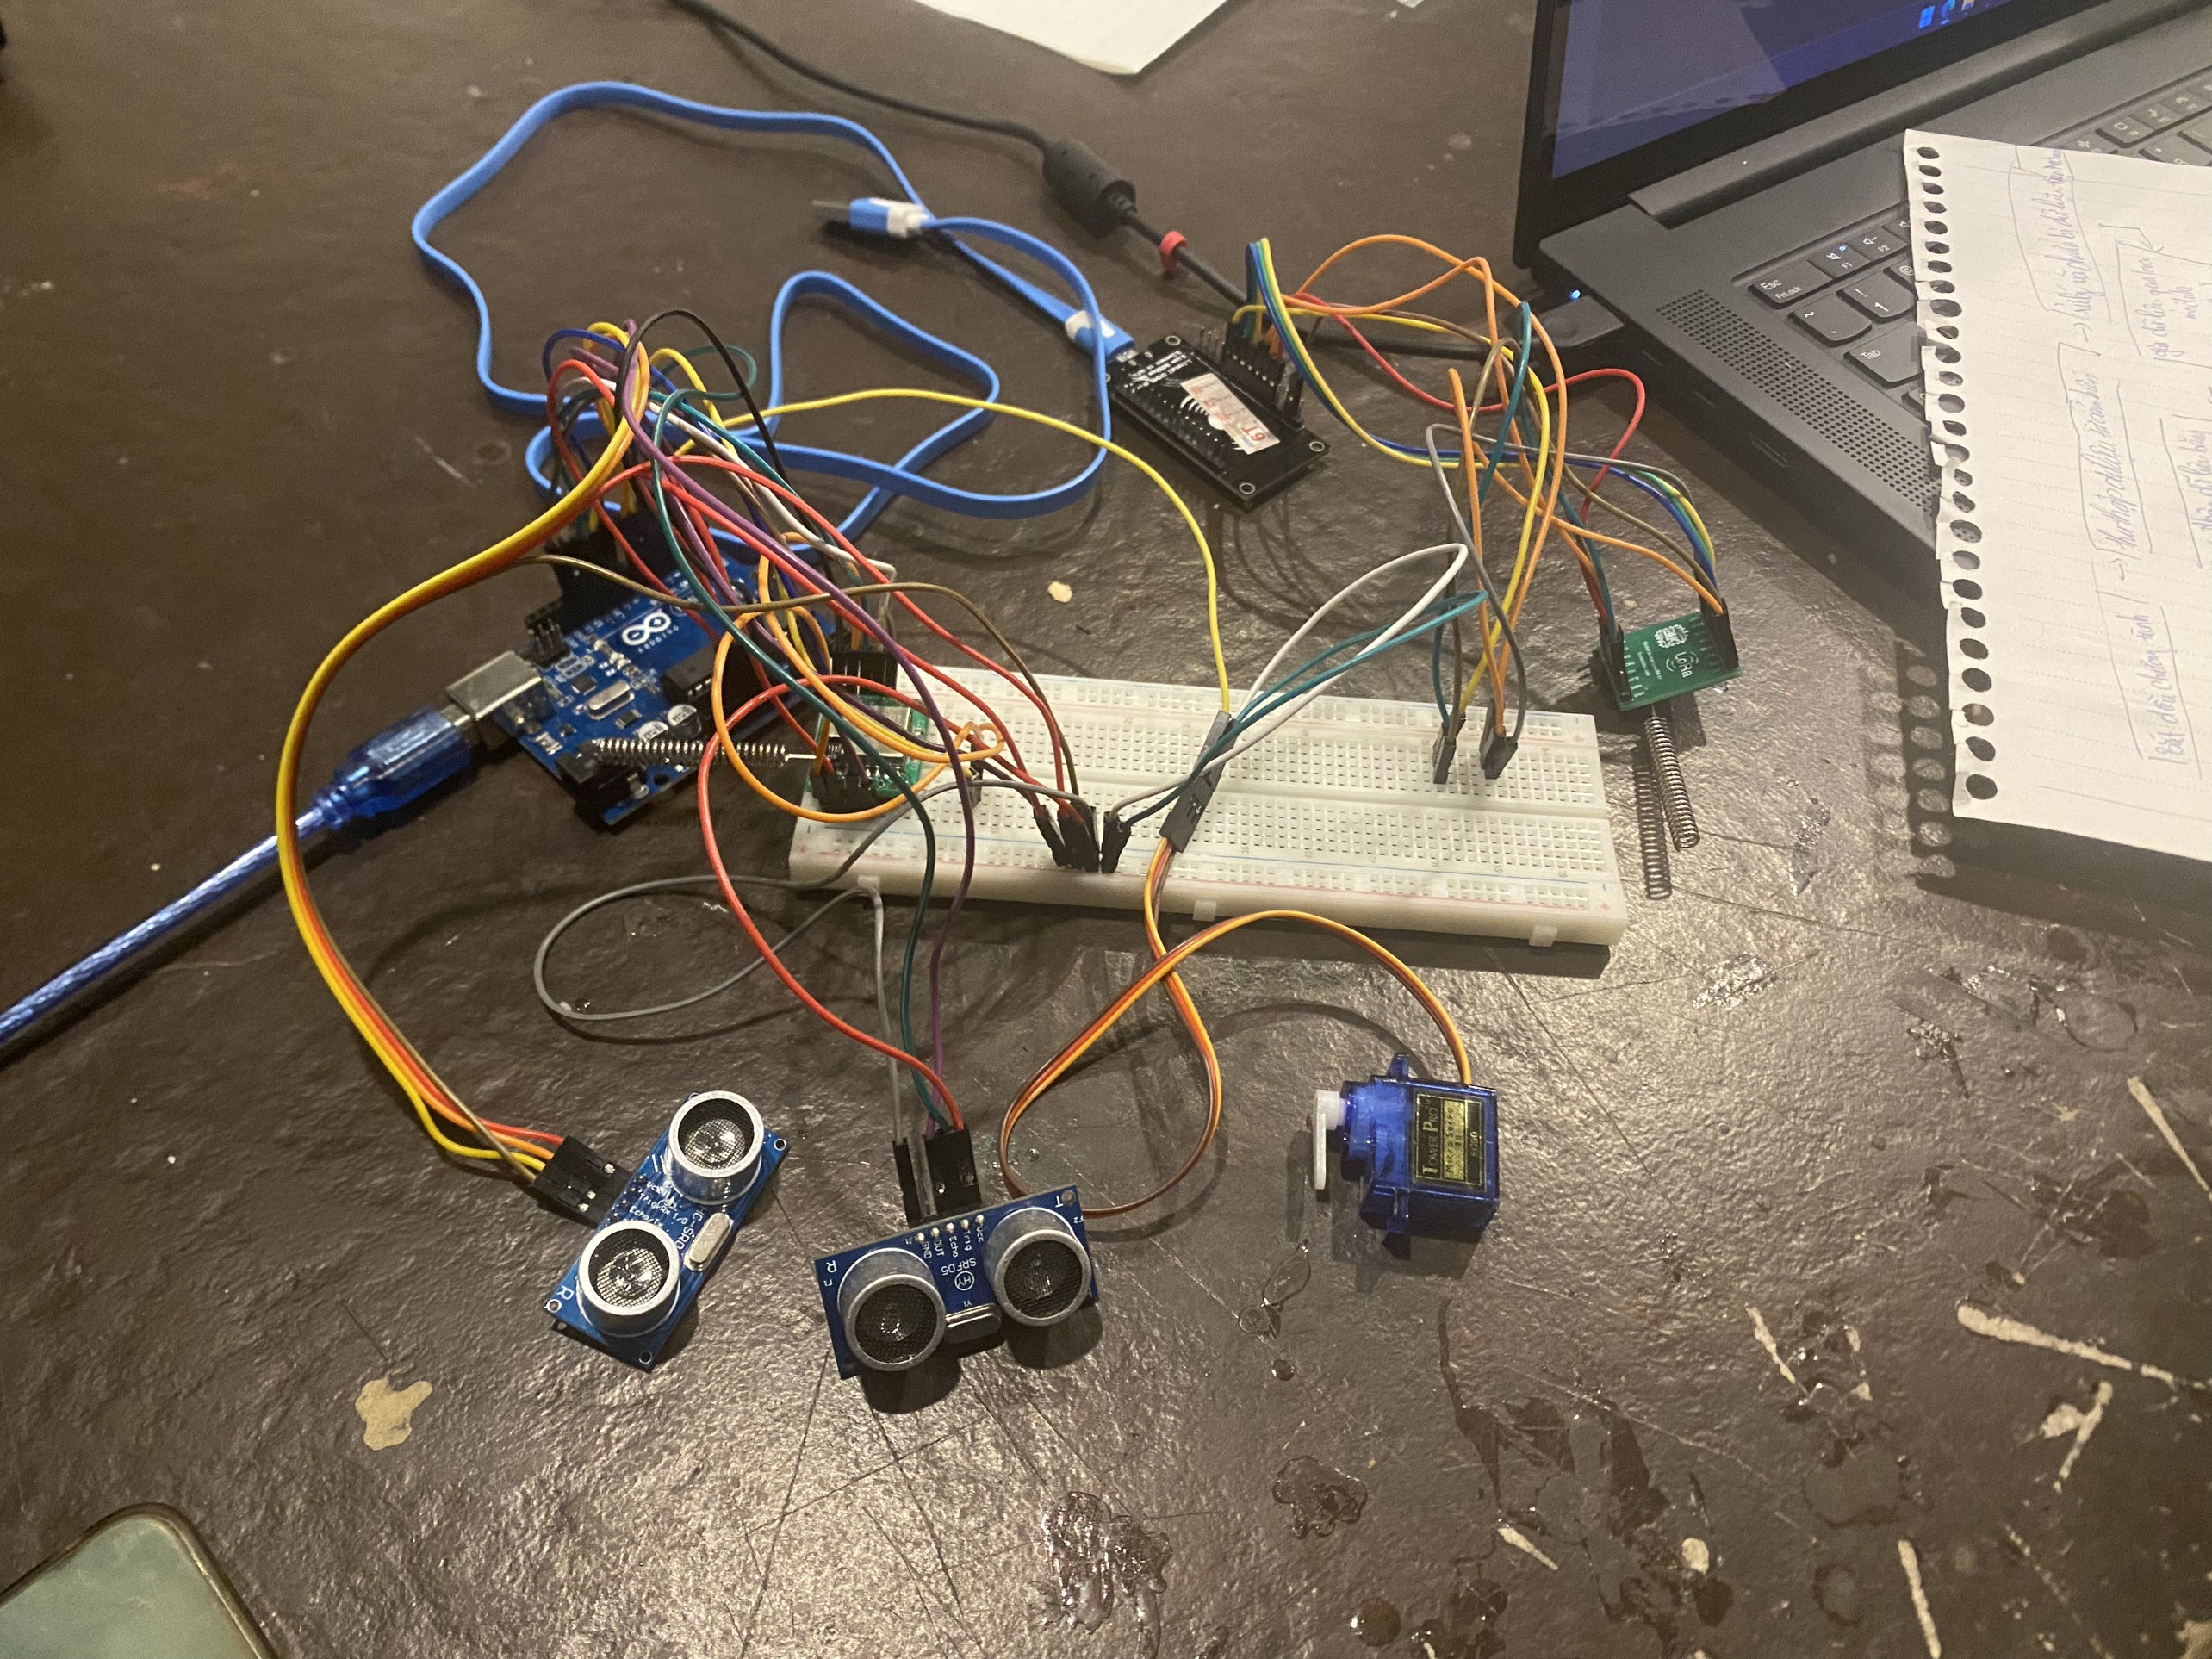
\includegraphics[width=3.8 in]{design1.png}}
B.1 Overview of the system
\end{center}

\begin{center}
\centerline{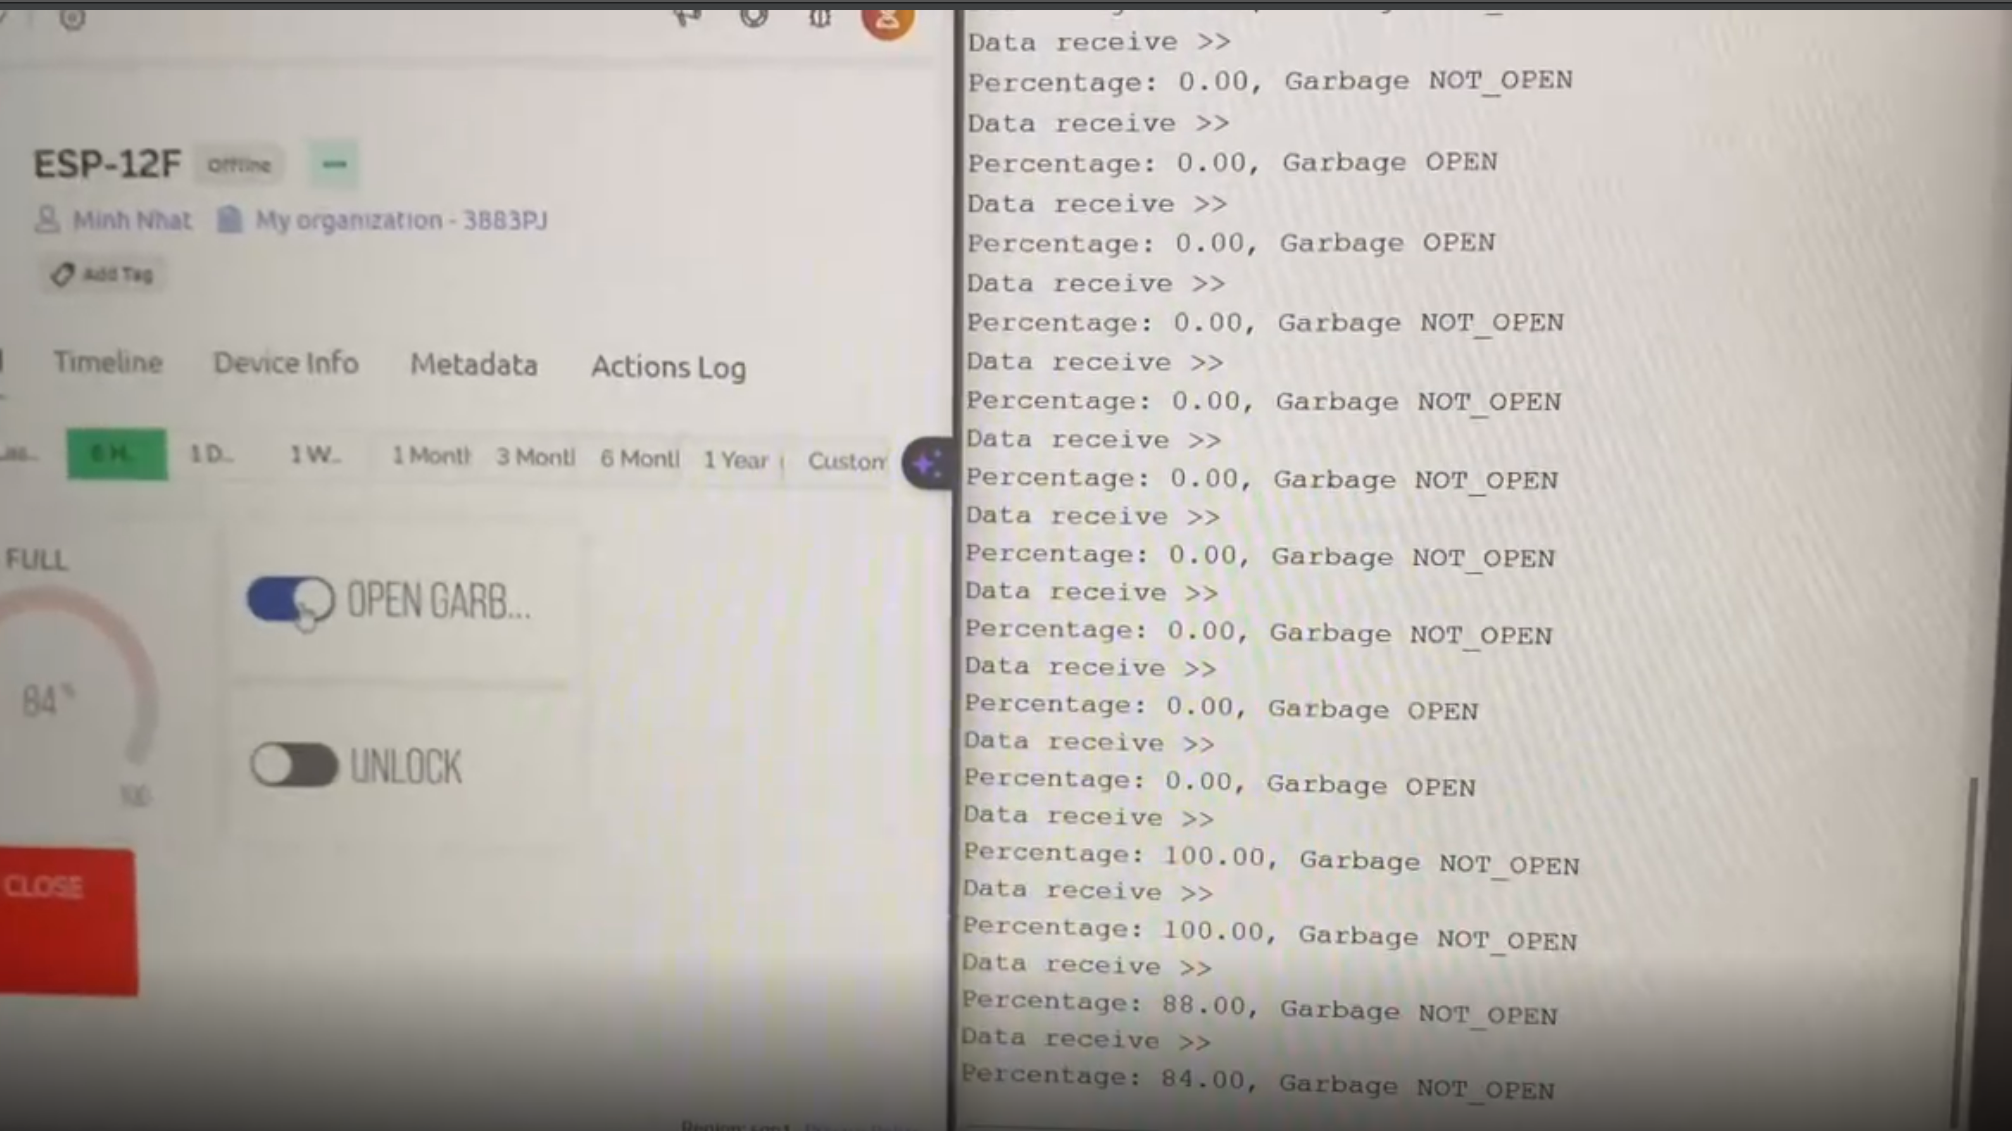
\includegraphics[width=3.8 in]{receive.png}}
\centerline{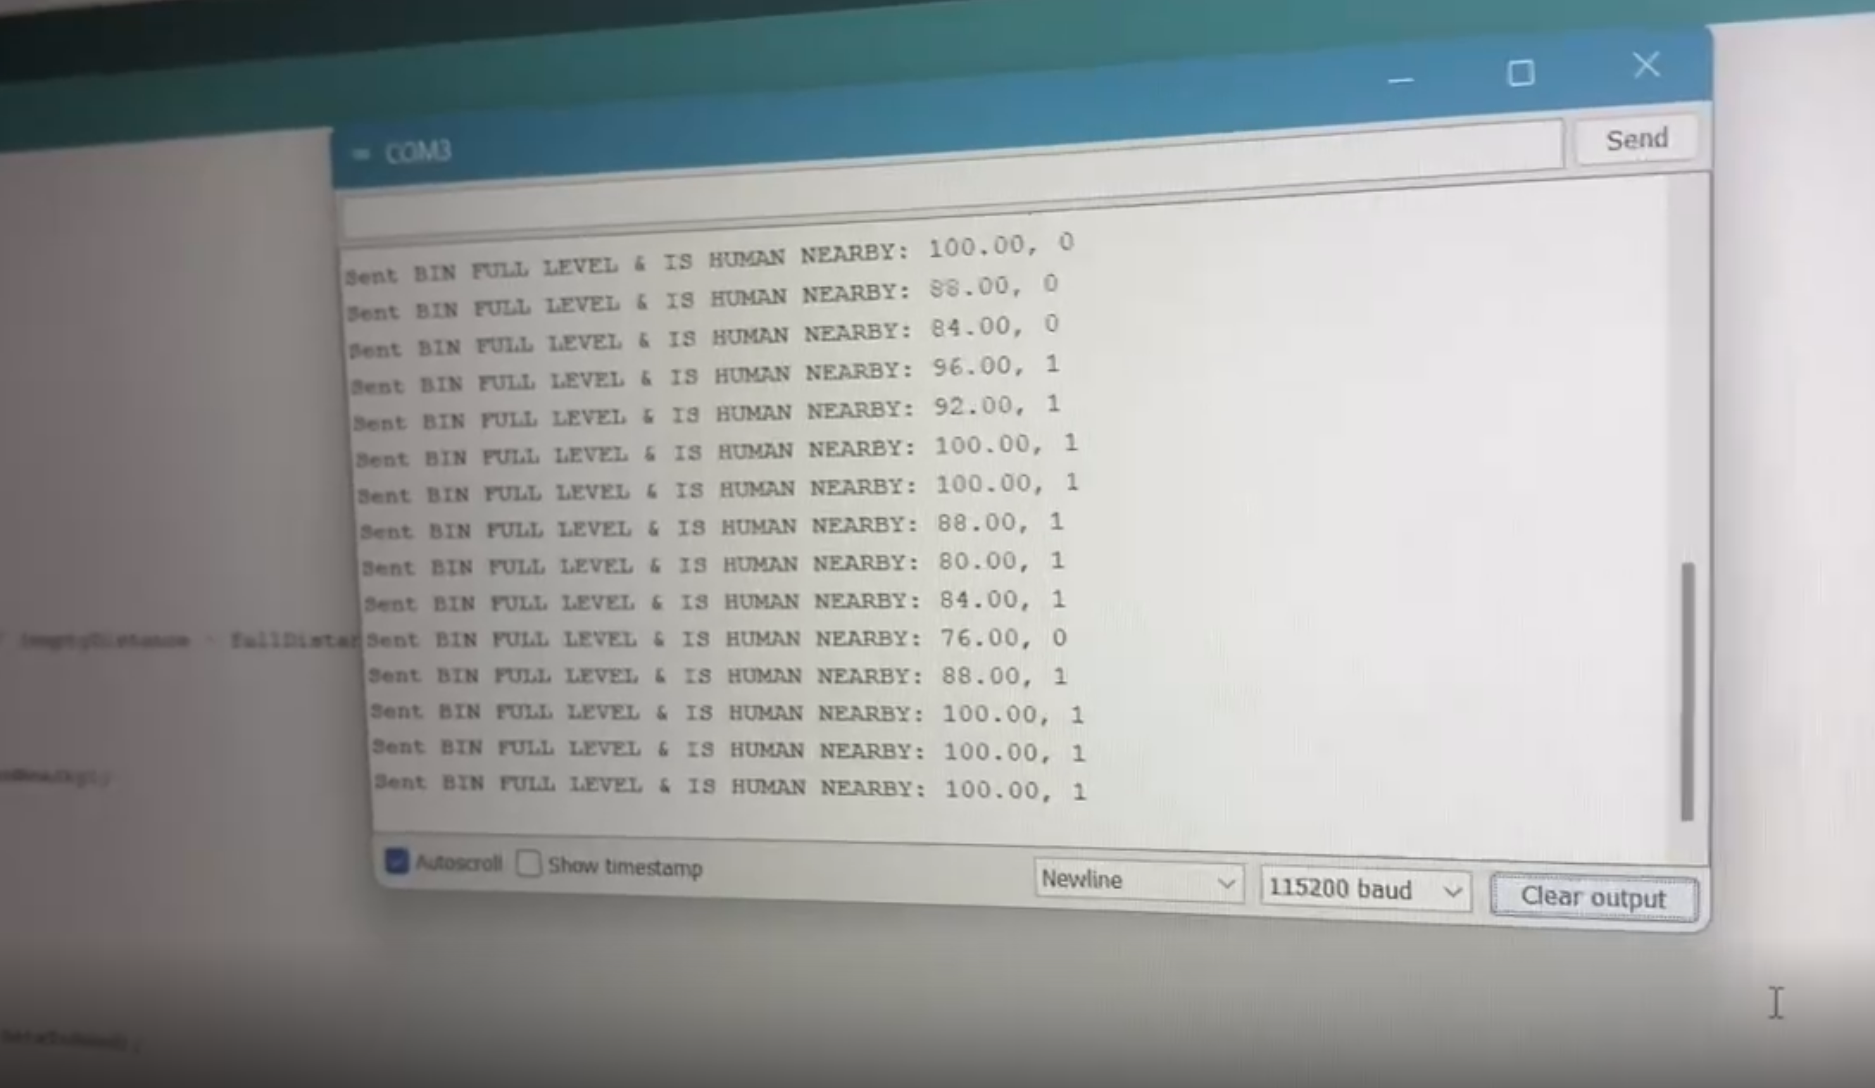
\includegraphics[width=3.8 in]{receive2.png}}
B.2 When the system collect data
\end{center}

\begin{center}
\centerline{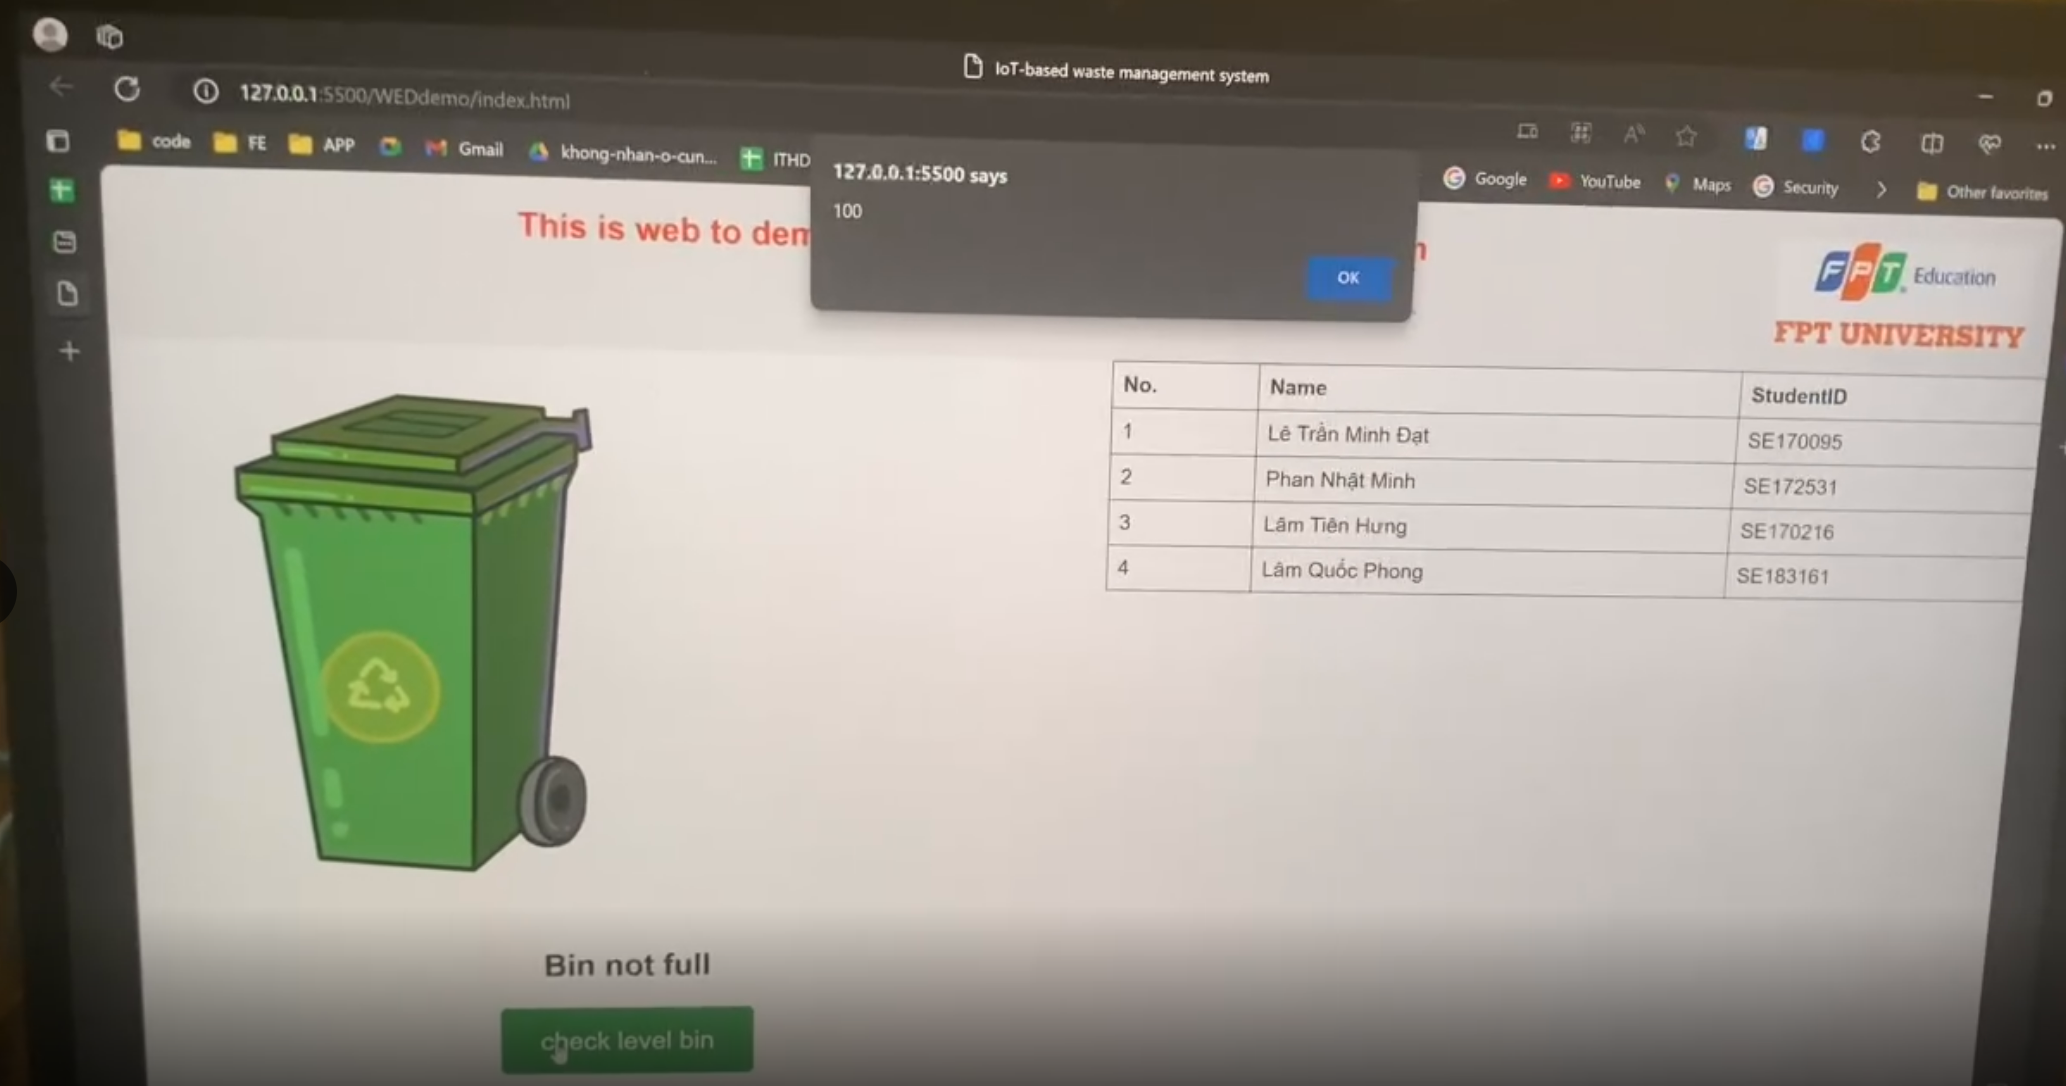
\includegraphics[width=3.8 in]{full.png}}
B.3 When the system is Full 
\end{center}

\begin{center}
\centerline{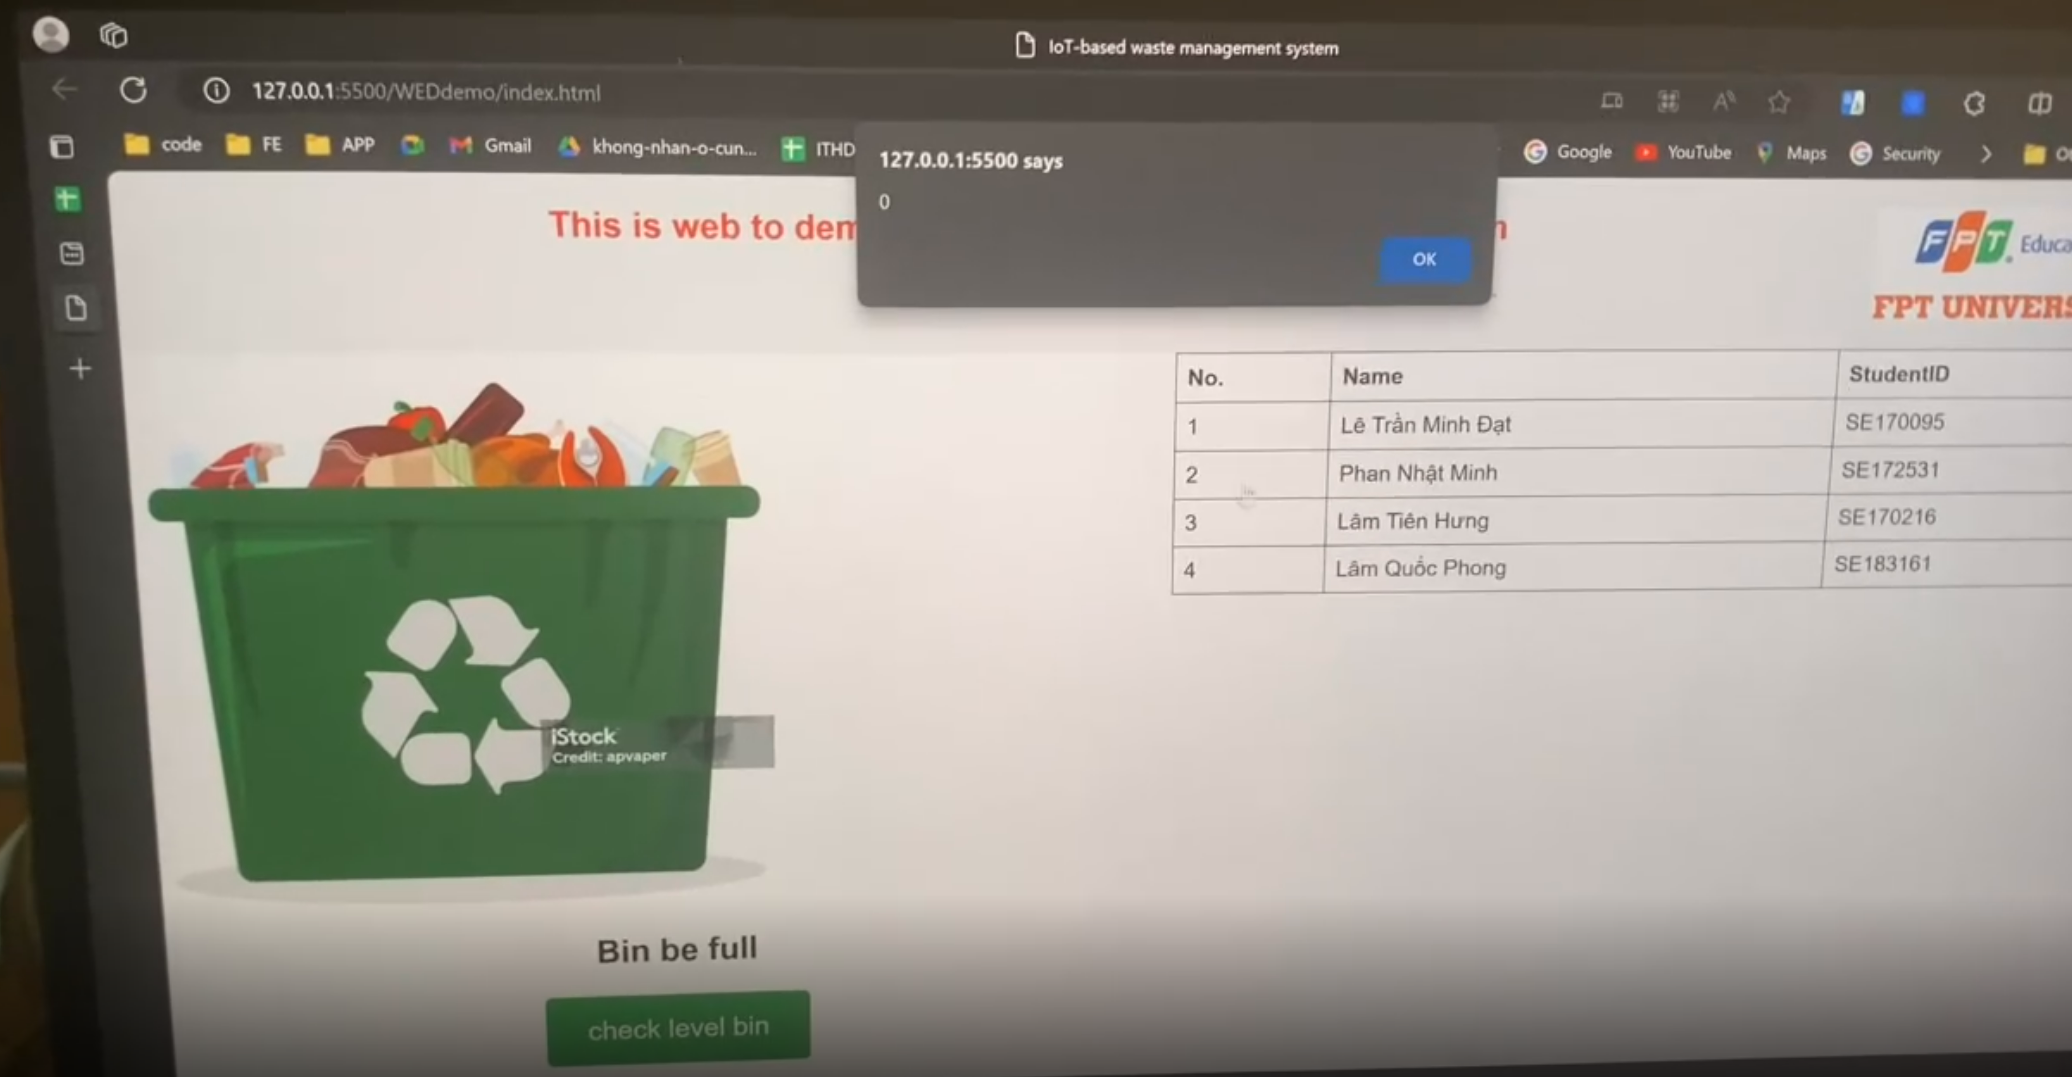
\includegraphics[width=3.8 in]{notfull.png}}
B.3 When the system is Not Full 
\end{center}

\subsection{Discussion}
The mix of Blynk 2.0 stage with the brilliant dustbin framework empowers constant observing of the fill level and controller abilities. Clients can get to the Blynk application from anyplace, permitting them to screen the fill level and get warnings on their cell phones or different gadgets. This continuous checking capacity further develops squander the board effectiveness by giving opportune data to planning assortment or removal exercises. Furthermore, the capacity to remotely control the framework offers accommodation and adaptability for clients, permitting them to start activities in view of the fill level information.

The Blynk 2.0 stage gives an easy to use connection point to cooperating with the brilliant dustbin framework. Users can easily control the system, set thresholds for notifications, and view the fill level data in a graphical format with the customizable Blynk app. The natural plan of the application improves the client experience and guarantees usability for people with changing specialized foundations. The smart dustbin system is more likely to be adopted and accepted in real-world situations thanks to this user-centric strategy.

During the implementation of the prototype, several challenges may have been encountered, such as connectivity issues, power management, or calibration of the ultrasonic sensor. These challenges highlight areas for future improvements. For example, exploring alternative connectivity options, such as LoRa or NB-IoT, could enhance the system's reliability and range. Power optimization techniques, such as sleep modes or energy harvesting, could be implemented to prolong the system's battery life. Additionally, fine-tuning the calibration of the ultrasonic sensor could improve the accuracy of fill level measurements.\\


\section{Conclusion}
The task yields include a practical shrewd dustbin framework with continuous fill level observing, IoT reconciliation with Blynk 2.0, visual and hear-able input systems, easy to understand point of interaction and control, information logging and examination capacities, and an indisputable report. The efficacy of waste management, enhanced user experience, and well-informed decision making in waste collection and disposal processes are all aided by these outputs.\\

\begin{table}[htbp]
\caption{Research Plan}
\begin{center}
\begin{tabular}{|c|l|l|c|}
\hline
\textbf{No}&\textbf{Task} & \textbf{Result form}& \textbf{Time schedule} \\
\hline
1 & Writing Abstract & Abstract & December 5, 2023 \\
\hline
3 & Writing Introduction & I. Introduction & December 5, 2023 \\
\hline
4 & Writing System Model and Design Block Diagram & II. Main Proposal & December 6, 2023 \\
\hline
5 & Writing Components and peripheral devices & II. Main Proposal & December 6, 2023 \\
\hline
6 & Writing Software programming, Programming Flowchart & II. Main Proposal & December 7, 2023 \\
\hline
7 & Writing III& III. Result and Discussion & December 7, 2023 \\
\hline
8 & Giving Final Conclusion& IV. Conclusion & December 8-10, 2023 \\
\hline
\end{tabular}
\label{tab1}
\end{center}
\end{table}
\emph{This is an example of a citation.}
For papers published in translation journals, please give the English citation first, followed by the original foreign-language citation \cite{dang2014her,anh2020waste,Khorov_2018,dang2015hybrid}  \cite{pham_jit}.

\bibliographystyle{IEEEtran}  %use this for IT
\bibliography{Bib_references}
\end{document}